\documentclass[12pt,letterpaper]{book}

\usepackage[export]{adjustbox}
\usepackage{amsmath}
\usepackage{amsfonts}
\usepackage{amssymb}
\usepackage[spanish,es-tabla]{babel}
\usepackage{booktabs}
\usepackage{caption}
\usepackage{fancyhdr}
\usepackage{framed}
\usepackage{geometry}
\usepackage{graphicx}
\usepackage[utf8]{inputenc}
\usepackage{listings}
\usepackage{titlesec}
\usepackage{xcolor}
\usepackage{courier}

\usepackage{etoolbox}

\definecolor{light-gray}{HTML}{FFFFFF}
\definecolor{java-comment}{rgb}{0,0.5,0}
\definecolor{java-keyword}{rgb}{0.13,0.13,1}
\definecolor{java-literal}{rgb}{0,0.6,0}
\definecolor{java-annotation}{rgb}{0.46,0.45,0.48}
\definecolor{java-string}{HTML}{CE7B00}
\definecolor{java-const}{HTML}{6600CC}


%	Cambia los margenes del documento
\geometry{left=23mm,top=20mm,right=23mm}
%	Modifica el formato del comando \section
\titleformat{\section}{\large\bfseries\raggedleft}{Lección \thesection}{1em}{}[{\titlerule[0.8pt]}]
%	Modifica el comando \chapter
\addto\captionsspanish{\renewcommand{\chaptername}{Unidad}}

%	Modifica el encabezado y pie de página
\pagestyle{fancy}
\fancyhf{}
\rhead{\chaptername : Elementos de Interfaces Gráficas}
\lhead{Tópicos Avanzados de Programación}
\rfoot{Página \thepage}
\lfoot{Rafael Rivera López}

%	Agrega espaciado en el interior del las filas de las tablas
\renewcommand{\arraystretch}{1.5}

%Para cambiar el grosor de la línea de encabezado o pie de página
%\renewcommand{\headrulewidth}{2pt}
\renewcommand{\footrulewidth}{0.5pt}

\renewcommand{\lstlistingname}{Código}



\lstset{
  aboveskip=3mm,
  belowskip=3mm,
  literate=
  {á}{{\'a}}1 {é}{{\'e}}1 {í}{{\'i}}1 {ó}{{\'o}}1 {ú}{{\'u}}1
  {Á}{{\'A}}1 {É}{{\'E}}1 {Í}{{\'I}}1 {Ó}{{\'O}}1 {Ú}{{\'U}}1
  {à}{{\`a}}1 {è}{{\`e}}1 {ì}{{\`i}}1 {ò}{{\`o}}1 {ù}{{\`u}}1
  {À}{{\`A}}1 {È}{{\'E}}1 {Ì}{{\`I}}1 {Ò}{{\`O}}1 {Ù}{{\`U}}1
  {ä}{{\"a}}1 {ë}{{\"e}}1 {ï}{{\"i}}1 {ö}{{\"o}}1 {ü}{{\"u}}1
  {Ä}{{\"A}}1 {Ë}{{\"E}}1 {Ï}{{\"I}}1 {Ö}{{\"O}}1 {Ü}{{\"U}}1
  {â}{{\^a}}1 {ê}{{\^e}}1 {î}{{\^i}}1 {ô}{{\^o}}1 {û}{{\^u}}1
  {Â}{{\^A}}1 {Ê}{{\^E}}1 {Î}{{\^I}}1 {Ô}{{\^O}}1 {Û}{{\^U}}1
  {œ}{{\oe}}1 {Œ}{{\OE}}1 {æ}{{\ae}}1 {Æ}{{\AE}}1 {ß}{{\ss}}1
  {ű}{{\H{u}}}1 {Ű}{{\H{U}}}1 {ő}{{\H{o}}}1 {Ő}{{\H{O}}}1
  {ç}{{\c c}}1 {Ç}{{\c C}}1 {ø}{{\o}}1 {å}{{\r a}}1 {Å}{{\r A}}1
  {€}{{\euro}}1 {£}{{\pounds}}1 {«}{{\guillemotleft}}1
  {»}{{\guillemotright}}1 {ñ}{{\~n}}1 {Ñ}{{\~N}}1 {¿}{{?`}}1,
  breaklines=true,
  breakatwhitespace=true,
  postbreak=\raisebox{0ex}[0ex][0ex]{\ensuremath{\color{red}\hookrightarrow\space}},
  language=Java,
  framesep=5pt,
  frame=Trbl,
  basicstyle=\scriptsize\ttfamily,
  columns=fullflexible,
  backgroundcolor=\color{light-gray},
  commentstyle=\color{java-comment},
  keywordstyle=\bfseries\color{java-keyword},
  stringstyle=\color{java-string},
  morecomment=[s][\color{gray}]{@}{\ },
  moredelim={[is][\bf]{\#bf}{\#bf}},
}

\fboxsep=6mm 	%Añade un espacio enter el marco y el contenido de un \fbox{}
\fboxrule=1pt 	%Modifica el grosor del marco de \fbox{}
 
 

\begin{document}
\chapter{Elementos de Interfaces Gráficas}


\section{Computación Gráfica}

\subsection{Esquema general de elementos gráficos}

Para ubicar los objetos gráficos se utiliza un sistema de coordenadas. En computación gráfica, el sistema de coordenadas es disinto al tradicional. Vease la imagen \ref{fig:coord-system} para una comparativa entre ambos sistemas.

\begin{figure}[!hbp] \centering \fboxsep=1mm 
\fbox{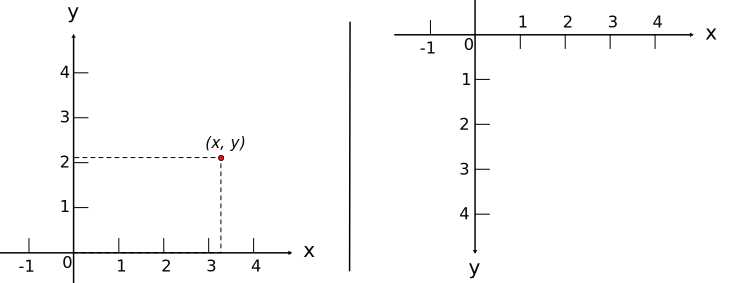
\includegraphics[width=0.9\textwidth]{images/coords}}
\caption{Izquierda: Sistema coordenado tradicional; Derecha: Sistema usado en computación gráfica}
\label{fig:coord-system}
\end{figure}

\subsubsection{Prism}

Prism es el componente de la arquitectura de JavaFX encargado de los trabajos de renderizado de gráficas. Posee un hilo de ejecución independiente para el renderizado, lo cual permite que un frame N sea renderizado mientras se está procesando el frame N+1 favoreciendo el desempeño general de las aplicaciónes.

\subsubsection{Pulsos}

\begin{center}
<<{\it \normalsize A pulse is an event that indicates to the JavaFX scene graph that it is time to synchronize the state of the elements on the scene graph with Prism.}>>
\end{center}

\hfill Java Documentation of Oracle\footnote{http://docs.oracle.com/javase/8/javafx/get-started-tutorial/jfx-architecture.htm\#JFXST788}\\

En pocas palabras, cuando un pulso sucede, JavaFX se encarga de renderizar la sección o el elemento gráfico que disparó el pulso. Hay que resaltar que los programadores no tienen que lidiar directamente con los pulsos, estos eventos son generados tras bambalinas por el propio sistema de gráficos de JavaFX.\\

Un ejemplo de un evento desencadenador de un pulso es el cambio de ubicación de un control o la adicción o remoción de un nodo (con una parte gráfica) a un gráfo de escena vivo\footnote{Un grafo de escena vivo es un grafo que está añadido a un objeto \texttt{Stage}.}.

\subsection{Canvas}

La clase \texttt{javafx.scene.canvas.Canvas} es una subclase de \texttt{Node} que funciona como un lienzo para trazar primitivas gráficas y dibujos en 2D, inclusive se pueden aplicar transformaciones a los trazos. La parte interna del canvas en que se pueden realizar los trazos se conoce como \textbf{contexto gráfico}.

\begin{itemize}

\item En JavaFX se utiliza un objeto como motor de interpretación de los trazos en el contexto gráfico (también se le conoce como brocha). La brocha es un objeto de la clase \texttt{javafx.scene.canvas.GraphicsContext}.

\item El método \texttt{\bf getGraphiscContext2D()} sirve para generar una brocha del canvas.

\end{itemize}

\begin{minipage}[c]{0.95\textwidth}
\lstinputlisting[
	caption=Estructura general para el manejo del contexto gráfico.,
]{source-codes/t-1-3-general-structure.java}
\end{minipage}

\subsection{Contexto Gráfico}

Como se mencionó previamente, el uso de un hilo de ejecución independiente da la ventaja de que, por un lado se puedan procesar los trazos mientras que por otro se realiza el renderizado de los gráficos.\\

La clase \texttt{GraphicsContext} realiza los trazos del canvas mediante un buffer\footnote{Un buffer de datos es un espacio de la memoria en un disco o en un instrumento digital reservado para el almacenamiento temporal de información digital, mientras que está esperando ser procesada. \hfill - \hfill Wikipedia}. Cada ocasión que se usa alguno de sus métodos de trazado, se colocan en el buffer los parámetros necesarios para renderizarse en la imagen del canvas al final de cada \textbf{pulso} en el hilo de renderizado.

\begin{figure}[!hbp] \centering \fboxsep=1mm 
\fbox{\includegraphics[width=0.5\textwidth]{images/t1-3_app-code-2}}
\caption{Ejemplo de trazado de primitivas gráficas.}
\label{fig:coord-system}
\end{figure}

\begin{minipage}[c]{0.95\textwidth}
\lstinputlisting[
	caption=Aplicación de demostración para el manejo del contexto gráfico., 
]{source-codes/t-1-3_main-code-2.java}
\end{minipage}

\begin{minipage}[c]{0.95\textwidth}
\lstinputlisting[
	caption=Clase auxiliar para la construcción de la interface., 
]{source-codes/t-1-3_code-2_GraphicContextPane.java}
\end{minipage}

\subsection{Primitivas Gráficas}

La clase GraphicsContext proporciona los siguientes métodos para presentar las primitivas gráficas:\\

\textbf{Trazos}
\begin{itemize} \footnotesize
\item void strokeLine(double x1, double y1, double x2, double y2)
\item void strokeRect(double x, double y, double w, double h)
\item void strokeOval(double x, double y, double w, double h)
\item void strokeRoundRect(double x, double y, double w, double h, double arcWidth, double arcHeight)
\end{itemize}

\textbf{Figuras con relleno}
\begin{itemize} \footnotesize
\item void fillRect(double x, double y, double w, double h)
\item void fillOval(double x, double y, double w, double h)
\item void fillRoundRect(double x, double y, double w, double h, double arcWidth, double arcHeight)
\end{itemize}

\begin{figure}[!hbp] \centering \fboxsep=1mm 
\fbox{\includegraphics[width=0.8\textwidth]{images/round-rect_oval}}
\caption{Izquierda: Cuadrado redondeado y sus parámetros; Derecha: Óvalo y sus parámetros.}
\label{fig:round-rect_oval}
\end{figure}

\subsubsection{Color}

Para definir un nuevo color de contorno o relleno de un trazo, se utilizan los métodos
\begin{center}
{\footnotesize \bf \texttt{setStroke(Paint p)}} y {\footnotesize \bf \texttt{setFill(Paint p)}}
\end{center}
respectivamente.

\begin{itemize}
\item Se pueden utilizar los colores definidos en la clase \texttt{javafx.scene.paint.Color} (\texttt{RED, MAGENTA, CYAN, BLACK, ...,} entre muchos otros).
	\begin{itemize} \footnotesize
	\item \texttt{gc.setStroke(Color.CYAN);}
	\item \texttt{gc.setFill(Color.ORANGE);}
	\end{itemize}
\item Se puede crear un color a partir de sus componentes RGB (rojo, verde y azul) y su opacidad.
	\begin{itemize} \footnotesize
	\item \texttt{gc.setStroke(new Color(0.4, 0.4, 0, 1));}
	\item \texttt{gc.setFill(new Color(0.4, 0.4, 0, 1));}
	\end{itemize}
	
\item Los componentes de color y la opacidad tienen valores entre 0 y 1.
\end{itemize}

\begin{minipage}[c]{0.95\textwidth}
\lstinputlisting[
	caption=Clase PrimitivesPane., 
]{source-codes/t-1-3_code-2_PrimitivesPane.java}
\end{minipage}

\subsection{Arcos}

\begin{itemize} \itemsep0em \footnotesize  
\item void strokeArc(double x, double y, double w, double h, double sa, double aa, ArcType closure)
\item void fillArc(double x, double y, double w, double h, double sa, double aa, ArcType closure)
\end{itemize}

\begin{description} \itemsep0em 
\item[ArcType] Indica como será el cierre del arco.
	\begin{enumerate} \itemsep0em 
	\item[ROUND: ] Cierra el arco con líneas que parten desde los puntos de inicio y fin y se conectan en el centro del arco.
	\item[CORD: ] Cierra el arco con una línea recta que conecta los puntos de inicio y fin.
	\item[OPEN: ] No cierra el arco.
	\end{enumerate}
\end{description}

\begin{figure}[!htp] \centering \fboxsep=1mm 
\fbox{\includegraphics[width=0.4\textwidth]{images/arc}}
\caption{Arco y sus parámetros.}
\label{fig:round-rect_oval}
\end{figure}


\begin{minipage}[c]{0.95\textwidth}
\lstinputlisting[
	caption=Clase ArcsPane., 
]{source-codes/t-1-3_code-2_ArcsPane.java}
\end{minipage}

\begin{figure}[!htp] \centering \fboxsep=1mm 
\fbox{\includegraphics[width=0.5\textwidth]{images/app_code-2_arcs}}
\caption{Canvas con arcos dibujados.}
\label{fig:arcs}
\end{figure}

\subsection{Polígonos y Poli-líneas}

\begin{itemize} \itemsep0em \footnotesize
\item void strokePolygon(double[] xPoints, double[] yPoints, int nPoints)
\item void fillPolygon(double[] xPoints, double[] yPoints, int nPoints)
\item void strokeLine(double x1, double y1, double x2, double y2)
\end{itemize}

\begin{minipage}[c]{0.95\textwidth}
\lstinputlisting[
	caption=Clase PolygonsPane., 
]{source-codes/t-1-3_code-2_PolygonsPane.java}
\end{minipage}

\begin{figure}[!htp] \centering \fboxsep=1mm 
\fbox{\includegraphics[width=0.5\textwidth]{images/app_code-2_polygons}}
\caption{Canvas con polígonos y poli-línea.}
\label{fig:polygons}
\end{figure}

\subsection{Texto e Imágenes}

\texttt{GraphicsContext} es capaz de dibujar texto e imágenes.

\begin{itemize} \itemsep0em \footnotesize
\item void strokeText(String text, double x, double y)
\item void strokeText(String text, double x, double y, double maxWidth)
\item void fillText(String text, double x, double y)
\item void fillText(String text, double x, double y, double maxWidth)
\item void drawImage(Image img, double x, double y)
\item void drawImage(Image img, double x, double y, double w, double h)
\item void drawImage(Image img, double sx, double sy, double sw, double sh, double dx, double dy, double dw, double dh)
\end{itemize}

Se puede especificar la fuente que se usará para escribir en el canvas mediante el método \texttt{setFont(Font f)}.

\begin{itemize}
\item Se puede crear una fuente a través de alguno de los constructores de la clase Font:
	\begin{itemize} \footnotesize
	\item \texttt{Font(double size)}
	\item \texttt{Font(String name, double size)}
	\end{itemize}
\item Se puede crear una fuente a través de alguno de los métodos estáticos de la clase Font:
	\begin{itemize} \footnotesize
	\item {\tt \textit{font}(String family)} 
	\item {\tt \textit{font}(double size)}
	\item {\tt \textit{font}(String family, double size)}
	\item {\tt \textit{font}(String family, FontPosture p, double size)}
	\item {\tt \textit{font}(String family, FontWeight w, double size)}
	\item {\tt \textit{font}(String family, FontWeight w, FontPosture p, double size)} 
	\end{itemize}
\item Se pueden usar las fuentes cargadas en la máquina o alguno de los cinco tipos de fuente base (SansSerif, Serif, Monospaced, Dialog y DialogInput).
\item FontWeight es un enumerado que puede ser: {\footnotesize \tt THIN, EXTRA\verb|_|LIGHT, LIGHT, NORMAL, MEDIUM, SEMI\verb|_|BOLD, BOLD, EXTRA\verb|_|BOLD, BLACK}.
\item FontPosture es un enumerado que puede ser: {\footnotesize \tt ITALIC, NORMAL}.
\end{itemize}



\begin{minipage}[c]{0.95\textwidth}
\lstinputlisting[
	caption=Clase TextImagesPane., 
]{source-codes/t-1-3_code-2_TextImagesPane.java}
\end{minipage}

\begin{figure}[!htp] \centering \fboxsep=1mm 
\fbox{\includegraphics[width=0.8\textwidth]{images/app_code-2_text-images}}
\caption{Canvas con texto e imagen.}
\label{fig:polygons}
\end{figure}



\end{document}
